\documentclass[11pt]{article}

\usepackage[margin=1in]{geometry}
\usepackage{booktabs}
\usepackage{tabularx}
\usepackage{array}
\usepackage{microtype}
\newcolumntype{Y}{>{\raggedright\arraybackslash}X}
\usepackage{tikz}
\usetikzlibrary{arrows.meta,backgrounds,calc,fit,positioning,shapes.multipart}
\usepackage[hidelinks]{hyperref}

\title{Task2View Pilot Study\\
Subjects, Models, and Experimental Conditions}
\author{}
\date{September 2026}

\begin{document}
\maketitle

\section{Pilot study}
This pilot checks whether a stakeholder goal and a repository can be turned into one architecture view, before a larger evaluation. Three conditions receive the same two systems and the same ten goals. The diagrams are in \texttt{comparison/}: folder~1 is the agent with the skill, folder~2 is the plain agent, and folder~3 is the pipeline. Folder~3 is the image set from Task2View architecture. Figure~\ref{fig:study} is the whole pilot: repositories, prompts, the three approaches with the model each one used, the views, and the review. Section~\ref{sec:results} is that last step. The pipeline diagrams were not in the review.

\begin{figure}[ht]
\centering
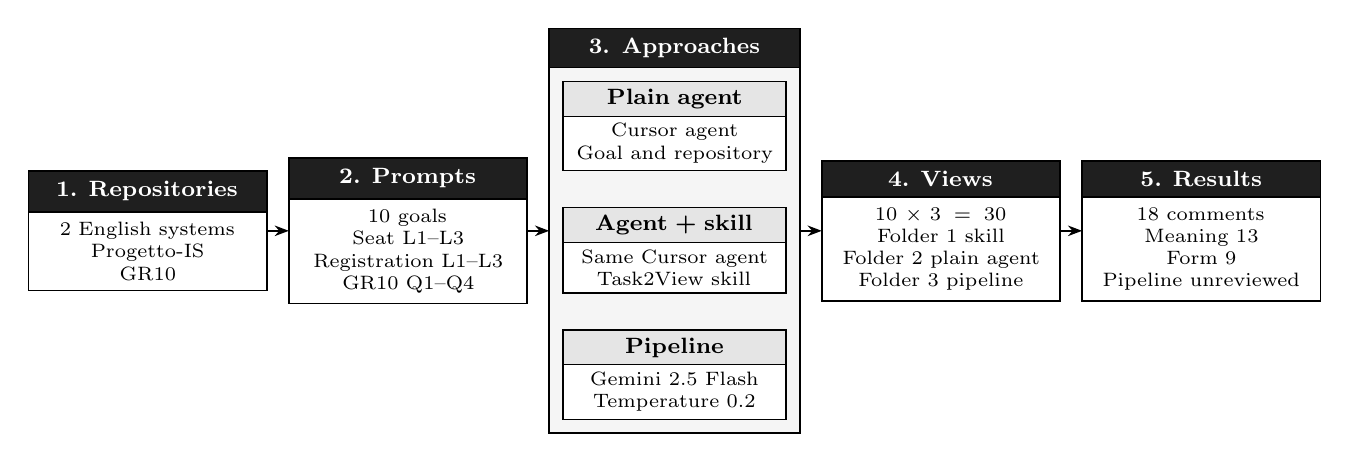
\begin{tikzpicture}[
  nohyph/.style={execute at begin node={\hyphenpenalty=10000\exhyphenpenalty=10000}},
  stage/.style={
    rectangle split, rectangle split parts=2,
    rectangle split part fill={black!88, white},
    rectangle split part align={center, center},
    draw, line width=0.6pt, align=center, font=\scriptsize,
    text width=2.78cm, inner xsep=3.5pt, inner ysep=3.5pt,
    outer sep=0pt, nohyph
  },
  method/.style={
    rectangle split, rectangle split parts=2,
    rectangle split part fill={black!10, white},
    rectangle split part align={center, center},
    draw, line width=0.45pt, align=center, font=\scriptsize,
    text width=2.62cm, inner xsep=3pt, inner ysep=2.5pt,
    outer sep=0pt, nohyph
  },
  arr/.style={-{Stealth[length=1.8mm]}, line width=0.6pt}
]
\node[method] (skill) {%
  \footnotesize\textbf{Agent + skill}%
  \nodepart{two}Same Cursor agent\\ Task2View skill};
\node[method, anchor=center] (plain) at ([yshift=1.58cm]skill.center) {%
  \footnotesize\textbf{Plain agent}%
  \nodepart{two}Cursor agent\\ Goal and repository};
\node[method, anchor=center] (pipe) at ([yshift=-1.58cm]skill.center) {%
  \footnotesize\textbf{Pipeline}%
  \nodepart{two}Gemini 2.5 Flash\\ Temperature 0.2};
\node[inner sep=5pt, outer sep=0pt, fit=(plain)(pipe)] (arms) {};
\path let \p1=($(arms.north east)-(arms.north west)$) in
  node[fill=black!88, text=white, font=\footnotesize\bfseries, anchor=south,
    inner ysep=3.5pt, inner xsep=0pt, outer sep=0pt, minimum width=\x1]
    at (arms.north) (appH) {3. Approaches};
\begin{scope}[on background layer]
  \fill[black!4] (appH.south west) rectangle (arms.south east);
  \fill[black!88] (appH.north west) rectangle (appH.south east);
\end{scope}
\draw[line width=0.6pt] (appH.north west) rectangle (arms.south east);
\draw[line width=0.6pt] (appH.south west) -- (appH.south east);
\coordinate (row) at ($(appH.north)!0.5!(arms.south)$);
\node[stage, anchor=east] (prompts) at ([xshift=-0.28cm]arms.west |- row) {%
  \textcolor{white}{\footnotesize\textbf{2. Prompts}}%
  \nodepart{two}10 goals\\ Seat L1--L3\\ Registration L1--L3\\ GR10 Q1--Q4};
\node[stage, anchor=east] (repos) at ([xshift=-0.28cm]prompts.west |- row) {%
  \textcolor{white}{\footnotesize\textbf{1. Repositories}}%
  \nodepart{two}2 English systems\\ Progetto-IS\\ GR10};
\node[stage, anchor=west] (views) at ([xshift=0.28cm]arms.east |- row) {%
  \textcolor{white}{\footnotesize\textbf{4. Views}}%
  \nodepart{two}\(10 \times 3 = 30\)\\ Folder 1 skill\\ Folder 2 plain agent\\ Folder 3 pipeline};
\node[stage, anchor=west] (results) at ([xshift=0.28cm]views.east |- row) {%
  \textcolor{white}{\footnotesize\textbf{5. Results}}%
  \nodepart{two}18 comments\\ Meaning 13\\ Form 9\\ Pipeline unreviewed};

\draw[arr] (repos) -- (prompts);
\draw[arr] (prompts) -- (arms.west |- row);
\draw[arr] (arms.east |- row) -- (views);
\draw[arr] (views) -- (results);
\end{tikzpicture}
\caption{Pilot study flow.}
\label{fig:study}
\end{figure}

\subsection{Subjects}
Both subjects are the English variants under \texttt{data\_points/}. Each fits in one model call. The ten goals are a developer changing seat booking and a tester covering registration, each at three levels of detail, plus four GR10 roles: architect, DevOps engineer, database engineer, and business analyst.

\begin{table}[h]
\centering
\small
\begin{tabularx}{\textwidth}{@{}lYY@{}}
\toprule
 & Progetto-IS & GR10 \\
\midrule
System & University library seat reservation & Municipal report management \\
Stack & Java 21, Swing + Spring Boot, JPA, MySQL & Java 23, Swing, JPA, MySQL; BCED packages \\
Size & 80 Java files, $\sim$10k LOC & 44 Java files, $\sim$11.8k LOC \\
Goals & Seat booking L1--L3; registration L1--L3 & Q1--Q4 \\
Reference & Design documentation & Visual Paradigm model \\
\bottomrule
\end{tabularx}
\caption{Pilot subjects.}
\label{tab:subjects}
\end{table}

\subsection{Models}
The pipeline uses one model for every phase call. The two agent conditions use one Cursor general-purpose agent. The skill is the only difference between those two arms. The agent run folders do not store a model id.

\begin{table}[h]
\centering
\small
\begin{tabularx}{\textwidth}{@{}YYYY@{}}
\toprule
Condition & Model & Setting & Role \\
\midrule
Pipeline & Gemini 2.5 Flash & temperature 0.2 & Every phase that calls a model \\
Agent, both arms & Cursor general-purpose agent & same model in both arms & Reads the repository and writes the view \\
\bottomrule
\end{tabularx}
\caption{Models in the pilot. Gemini is the Google AI Studio default (\texttt{GEMINI\_MODEL}, otherwise \texttt{gemini-2.5-flash}).}
\label{tab:models}
\end{table}

\subsection{Conditions}
The repository and the goal stay fixed.

\noindent\textbf{Plain agent} (\texttt{comparison/folder2}).
The agent receives the repository path and the goal. It is given neither the skill, the viewpoint catalog, nor the pipeline. It writes a PlantUML view, and on a few goals a short note.

\noindent\textbf{Agent with the Task2View skill} (\texttt{comparison/folder1}).
The same kind of agent follows \texttt{task2view-skill}. It interprets the stakeholder, chooses one catalog viewpoint, binds that viewpoint's grain, and publishes the phase JSON plus a diagram. It does not run \texttt{task2view}.

\noindent\textbf{Pipeline} (\texttt{comparison/folder3}, \texttt{runs/pilot}).
PageRank on the uses/calls graph (Aider RepoMap, damping 0.85) proposes files, and a token budget keeps a subset. This batch kept 2--8 files. The phases are separate Gemini calls:
\begin{enumerate}
\item interpret the stakeholder and task;
\item write architectural questions;
\item choose one catalog viewpoint and its diagram language;
\item build the graph, scope files, and write an analysis plan;
\item extract claims from the files named in that plan;
\item reconcile questions with the claims, without redrawing the view;
\item publish a view model from that evidence;
\item validate names against the scoped graph and emit PlantUML.
\end{enumerate}
Each pilot run records \texttt{scope\_strategy: pagerank} and an \texttt{architecture\_evidence\_model.json}.

\begin{table}[h]
\centering
\small
\begin{tabularx}{\textwidth}{@{}lYYY@{}}
\toprule
 & Plain agent & Agent + skill & Pipeline \\
\midrule
Who decides & The agent & One agent, one catalog viewpoint & A Gemini call per phase \\
Repository & Read as the agent chooses & Read after the viewpoint is fixed & PageRank, then a token budget (2--8 files here) \\
Output & Diagram, sometimes a note & Phase JSON + diagram & Phase JSON, evidence model, diagram, validation report \\
Model & Cursor agent & Same Cursor agent & Gemini 2.5 Flash, temperature 0.2 \\
\bottomrule
\end{tabularx}
\caption{The three pilot conditions.}
\label{tab:conditions}
\end{table}

\section{Results}
\label{sec:results}
A reviewer wrote one comment on each of the ten goals for the skill agent and the plain agent, plus one comment covering all three seat-booking diagrams of the plain agent: 18 comments in \texttt{comparison\_review.txt}. Seven fit the goal, five are partial, and six miss it. Short goals are the ones accepted. The detailed prompts are the ones rejected. The pipeline diagrams in folder~3 were not reviewed.

The seven themes fall into two buckets. \textbf{Meaning} is whether the diagram says the right architectural thing. \textbf{Form} is whether it is drawn as a proper view. Thirteen comments raise a meaning issue. Nine raise a form issue. Six raise both. Two plain-agent diagrams raise neither: the DevOps deployment view, and registration at the shortest prompt.

\begin{table}[h]
\centering
\small
\begin{tabularx}{\textwidth}{@{}llYY@{}}
\toprule
Bucket & Theme & Skill & Plain agent \\
\midrule
Meaning & Second view: structure and behavior in one picture & 3 & 3 \\
Meaning & Grain: too coarse, or several levels at once & 2 & 3 \\
Meaning & Layers: components with no package around them & 4 & 0 \\
Meaning & Names: not a source element, or parts the goal did not ask for & 1 & 3 \\
\midrule
Form & Notation: boxes, symbols, stereotypes & 2 & 4 \\
Form & Placement: a fact drawn on the wrong mark & 2 & 0 \\
Form & Layout: arrows or arrangement, content otherwise accepted & 1 & 1 \\
\bottomrule
\end{tabularx}
\caption{Comment blocks that raise each theme. One comment can raise more than one theme. Counts are out of 10 skill comments and 8 plain-agent comments.}
\label{tab:themes}
\end{table}

\paragraph{Meaning.}
\textit{Second view} (6). The reviewer wants a component diagram for the parts and a sequence diagram for the order of calls. Registration L2--L3 and seat booking L2--L3, in both conditions.
\textit{Grain} (5). The level of detail does not follow the prompt. The longest registration request to the skill agent produced the coarsest picture. The plain agent mixes code snippets with subsystems.
\textit{Layers} (4). The boxes are a flat list. The reviewer wants Boundary, Control, Entity, and Database around them. All four comments are on the skill agent. The architect comment asks for the GUI pieces to sit inside one higher package.
\textit{Names} (4). A box is not a source element, or the diagram adds a part the goal did not ask for. Three of the four are the plain agent. Registration L2 draws a box named ``boundary Autenticazione POST /api/auth/registrazione''.

\paragraph{Form.}
\textit{Notation} (6). The content may be useful, and it is not drawn as the view it claims to be. Four of the six are the plain agent. The architect diagram is closer to a flowchart than a component view. The skill agent's database diagram uses aggregation symbols for the wrong relation.
\textit{Placement} (2). The fact is in the diagram and attached to the wrong mark. Both comments are on the skill agent. Responsibilities are written on edges. On the database goal, \texttt{id\_cittadino} is the label of a line between two classes, where the reviewer expects an attribute.
\textit{Layout} (2). The content is accepted. An arrow has no source on the skill agent's deployment view, and the plain agent's analyst diagram is hard to follow.

The skill agent is the condition that drops layers and misplaces facts. The plain agent is the condition that drops notation and grounded names. On registration at the shortest prompt, and on the persistence core of the database goal, the plain agent is the diagram the reviewer prefers.

Three skill comments on Progetto-IS name the other feature. Registration L1 and L2 are discussed as seat booking. Seat booking L3 is discussed as registration. The theme in each comment still holds. Those three sentences should be checked against the diagram before they are cited for a specific goal.

\end{document}
